%%%%%%%%%%%%%%%%%%%%%%%%%%%%%%%%%%%%%%%%%
% Short Sectioned Assignment
% LaTeX Template
% Version 1.0 (5/5/12)
%
% This template has been downloaded from:
% http://www.LaTeXTemplates.com
%
% Original author:
% Frits Wenneker (http://www.howtotex.com)
%
% License:
% CC BY-NC-SA 3.0 (http://creativecommons.org/licenses/by-nc-sa/3.0/)
%
%%%%%%%%%%%%%%%%%%%%%%%%%%%%%%%%%%%%%%%%%

%----------------------------------------------------------------------------
%	PACKAGES AND OTHER DOCUMENT CONFIGURATIONS
%----------------------------------------------------------------------------

\documentclass[paper=a4, fontsize=11pt]{scrartcl} % A4 paper and 11pt font size

\usepackage[T1]{fontenc} % Use 8-bit encoding that has 256 glyphs
\usepackage{fourier} % Use the Adobe Utopia font for the document - comment this line to return to the LaTeX default
\usepackage[english]{babel} % English language/hyphenation
\usepackage{amsmath,amsfonts,amsthm} % Math packages

\usepackage{lipsum} % Used for inserting dummy 'Lorem ipsum' text into the template

\usepackage{graphicx} % Used for including graphics
\usepackage{caption}
\usepackage{subcaption}
\usepackage{listings}
\usepackage{sectsty} % Allows customizing section commands
\allsectionsfont{\centering \normalfont\scshape} % Make all sections centered, the default font and small caps

\usepackage{fancyhdr} % Custom headers and footers
\usepackage{cite}
\bibliographystyle{plain}
\pagestyle{fancyplain} % Makes all pages in the document conform to the custom headers and footers
\fancyhead{} % No page header - if you want one, create it in the same way as the footers below
\fancyfoot[L]{} % Empty left footer
\fancyfoot[C]{} % Empty center footer
\fancyfoot[R]{\thepage} % Page numbering for right footer
\renewcommand{\headrulewidth}{0pt} % Remove header underlines
\renewcommand{\footrulewidth}{0pt} % Remove footer underlines
\setlength{\headheight}{13.6pt} % Customize the height of the header

\numberwithin{equation}{section} % Number equations within sections (i.e. 1.1, 1.2, 2.1, 2.2 instead of 1, 2, 3, 4)
\numberwithin{figure}{section} % Number figures within sections (i.e. 1.1, 1.2, 2.1, 2.2 instead of 1, 2, 3, 4)
\numberwithin{table}{section} % Number tables within sections (i.e. 1.1, 1.2, 2.1, 2.2 instead of 1, 2, 3, 4)

\setlength\parindent{0pt} % Removes all indentation from paragraphs - comment this line for an assignment with lots of text

%----------------------------------------------------------------------------
%	TITLE SECTION
%----------------------------------------------------------------------------

\newcommand{\horrule}[1]{\rule{\linewidth}{#1}} % Create horizontal rule command with 1 argument of height

\title{
\normalfont \normalsize
\textsc{King Abdullah University of Science and Technology\\
        Division of Mathematical and Computer Sciences and Engineering\\
        Design and Analysis of Algorithms} \\ [25pt] % Your university, school and/or department name(s)
\horrule{0.5pt} \\[0.4cm] % Thin top horizontal rule
\Large Midterm Project Report\\
\huge Diverse Approaches to Exact Pattern Matching
\horrule{2pt} \\[0.5cm] % Thick bottom horizontal rule
}

\author{Affara, Lama\\
        Almansour, Durrah\\
        Al-Shedivat, Maruan\\
        Chen, Gui\\
        Fujii, Chisato\\
        Rapakoulia, Trisevgeni}


\date{\normalsize\today} % Today's date or a custom date


\begin{document}
\begin{titlepage}
\maketitle
\thispagestyle{empty}
\clearpage
\end{titlepage}

%----------------------------------------------------------------------------
%    INTRODUCTION
%----------------------------------------------------------------------------

\section{Introduction}
Pattern matching remains to this day an extensively studied problem. The exponential growth of computing and data collection has increased the need for a more efficient solution to this problem. Pattern matching is applied in a wide range of disciplines such as Database queries, Text editors, two dimensional mesh, Bioinformatics, music content retrieval, MS word spell checker, digital libraries, and search engines.\\

One optimal algorithm that can be applied to all such applications which include different data formats has not been established. Therefore, we intend to test the performance of three different algorithms: Aho-Corasick, Suffix-tree, and Boyer-Moore algorithms. We will theoretically analyse and compare the time complexities of the above three algorithms. We will also apply them on texts, patterns, and alphabets of various types and lengths.\\

Pattern matching can be defined as follows\cite{intro}: Given a text T of length n and a pattern P of length k over some alphabet $\Sigma$, where n > k, the exact pattern matching problem consists of finding all occurrences z of the pattern P in the text T.\\

For example, let p = aba and t = abaababa over alphabet $\Sigma$ = \{a,b\}. As illustrated in Figure \ref{matching}, three occurrences of the considered pattern appear in the text, at locations 1, 4, and 6.

\begin{figure}[h!]
\centering
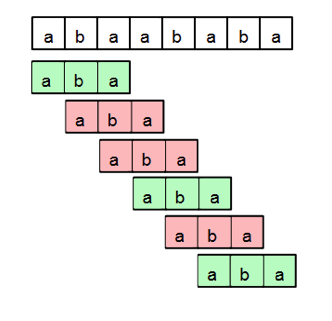
\includegraphics[width=0.6\textwidth]{figures/matching.png}
\caption{pattern matching instance}
\label{matching}
\end{figure}

A variety of algorithms have been developed for exact pattern matching, the most famous of which are presented in Figure \ref{algorithms}:

\begin{figure}[h!]
\centering
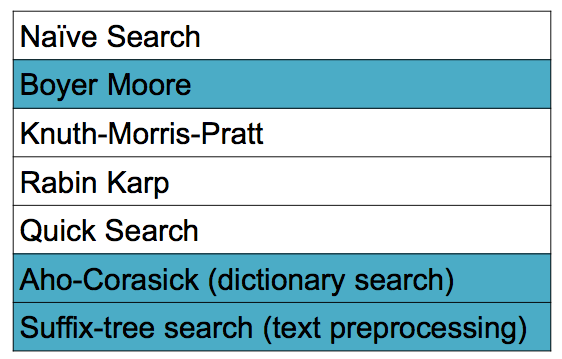
\includegraphics[width=0.4\textwidth]{figures/algorithms.png}
\caption{Algorithms for exact pattern matching}
\label{algorithms}
\end{figure}

\section{Boyre Moore}
Boyre Moore algorithm \cite{bm_fast} searches for all the occurrences of a pattern in a text. It is in some way similar to the naive search algorithm. Initially, it aligns the first character in P with the first character in T. The algorithm then compares characters between P and T sequentially from right to left. Once a mismatch occurs, a shift rule is applied thus moving the pattern by $s\ge 1$. The algorithm is basically divided into two stages: preprocessing and searching. There are different preprocessing approaches in the literature such as Bad Character Rule and Good Suffix Tree \cite{bm_tbc}. We decided to choose the extended Bad Character rule due to its simplicity and applicability to our dataset. In the following sections, we describe the two stages of the algorithm.

\begin{figure}[h!]
\centering
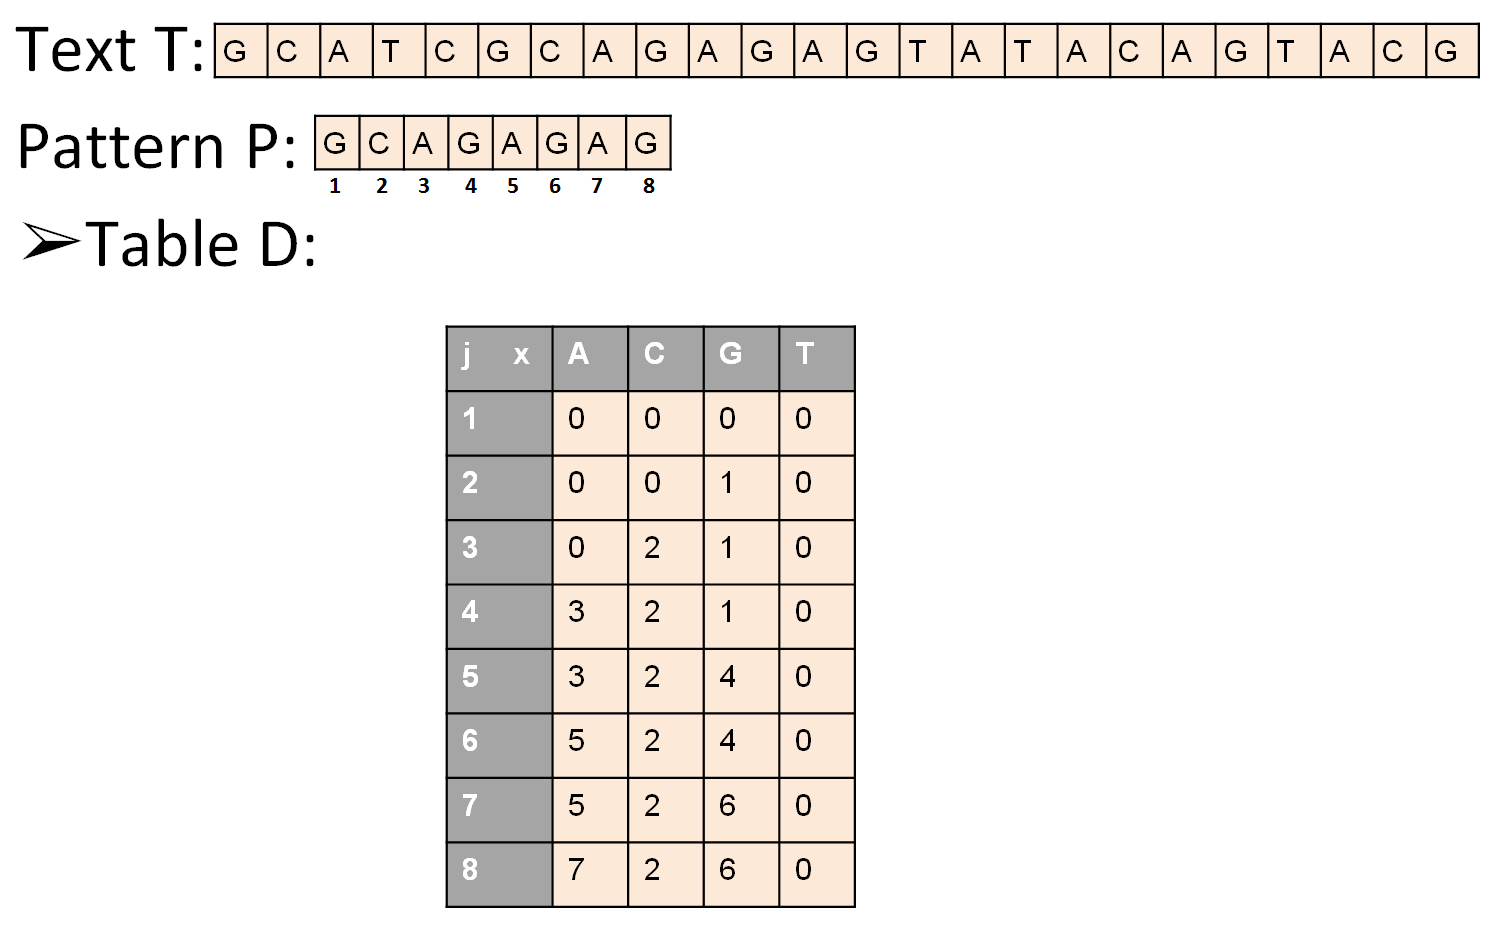
\includegraphics[width=0.8\textwidth]{figures/Example_Table.png}
\caption{Table of preprocessing phase}
\label{table}
\end{figure}

\subsection{Preprocessing Stage}
In the preprocessing stage, the algorithm makes use of the alphabet $\Sigma$ and the pattern P. A two dimensional table D is constructed by processing the pattern according to the available alphabet. D is of size $k\times|\Sigma|$ where for each mismatch index in P, the position of rightmost occurrence of a character in $\Sigma$ is stored. Figure \ref{table} shows an example of the table stored by processing the pattern GCAGAGAG based on the DNA alphabet=\{A,C,G,T\}. Starting from the last row corresponding to a mismatch occurring at position i=k in P, i=8 for this example, the algorithm scans P to find the rightmost index of the given character. In the below example, the last occurrence of A before position 8 is 7, G is 6, C is 2, and T is 0. It is important to note here that if a character does not exist in the pattern, its position in the table is always 0. The algorithm iterates from i=k to 1. If the mismatch occurs in position i-1, the algorithm updates only the value for the specific character placed in this position, A for this example, and all the other values remain the same as D[i,x]. The last occurrence of A before position 7 is 5, while G, C, and T stay the same.


\subsection{Searching Phase}
In the searching phase, the algorithm shifts the pattern and sequentially matches it with the aligned text. Starting from the rightmost character in P, the algorithm checks the aligned character in T. If the pair of characters are matching, it sequentially continues the check to the next left character. If a mismatch occurs at position j in P, the algorithm shifts P according to the mismatched character x in the text. For example, if at position j, the text contains a character that is not found in P, the pattern is shifted by j. However, if the mismatched character is found in P, the pattern is shifted by j-i, where i corresponds to the rightmost occurrence of this character in P. The index i of the last occurrence is retrieved from table D (i=D[j,x] where x is the character in the text). Figure \ref{search} shows the searching phase for the example shown in the previous section. The pseudocode of Boyre Moore algorithm is shown below.\\
\begin{lstlisting}
Algoritm: BMMatch(T, P):
Input: Text T (n characters) and pattern P (k characters)
Output: List I of indexes of occurences of P in T

D=Preprocess(P)
l=k
j=k
z=0
repeat
    if P[j] = T[l] then
        if j = 0 then
            I[z]=l;
	    z=z+1
        else {check next character}
            l = l - 1
            j = j - 1
    else { P[j] <> T[l] shift the pattern}
        x=T[l]
	i=D[j,x]
	l = l + k - j - 1 {reset l to position of P in T}
        l=l+ j - i
        j =k
until l > n
return "There is no substring of T matching P."
\end{lstlisting}

\begin{figure}[h!]
\centering
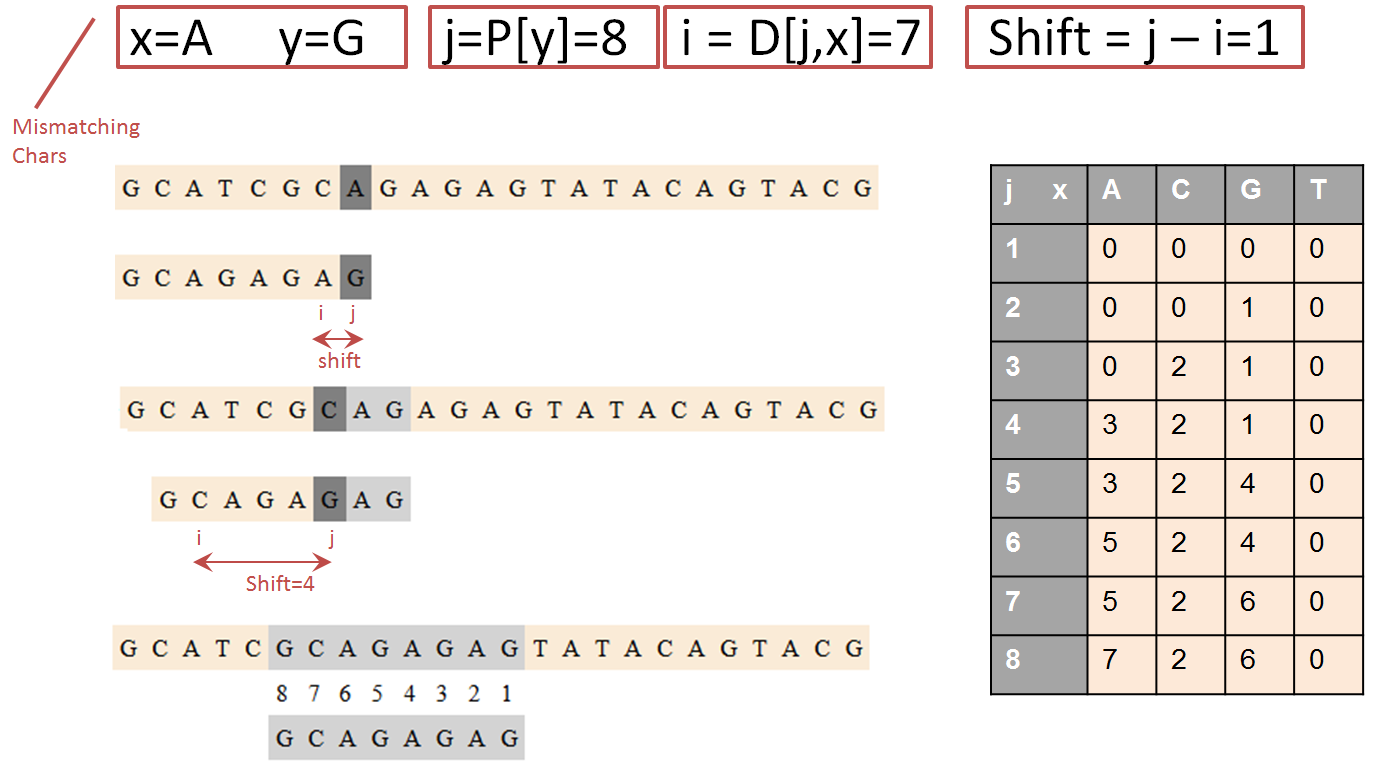
\includegraphics[width=0.8\textwidth]{figures/searching_phase.png}
\caption{Searching Phase}
\label{search}
\end{figure}


\subsection{Complexity}
In this section we show the time complexity for both the preprocessing and searching phases of the algorithm. For the preprocessing stage, a table of $k\times|\Sigma|$ is stored in memory, so the space complexity is O($k\times|\Sigma|$). Initially, the first row is initialized to zeros. At each step, one value is updated in the table and the rest of the values are copied from the row before it. So at each step i<k, $|\Sigma|$ operations are done. Thus, the preprocessing time complexity is O($k\times|\Sigma|$). For the searching phase, the text T is compared to pattern P from right to left. The worst time occurs when the shifts are only one character at a time and the algorithm would be similar to naive search with a complexity of O($k\times n$). However, the shifts employed by this algorithm allow it to have a sublinear complexity especially in the case of large alphabet and random strings.

\section{Dataset}
We will apply these algorithms on an available dataset of DNA sequences and natural language text, to find specific sequence motifs in the first, and words and phrases in the latter. With regards to the biological dataset, we selected  the DNA sequence of  human chromosome 1 in fasta format as a searching test. The DNA alphabet consists of four elements, $\Sigma$ = \{A, C, G, T\}, that represent  the four nitrogenous bases. We also chose three different patterns for our experimental measurements. As for the natural language data set, we will search for specific phrases of varying lengths. We will compare the performance in the two data sets to highlight the effect of the size of the alphabet and pattern length.
Applying the algorithms on these datasets will show practical results on the analytical complexities that we examined and the difference in performance of the three above mentioned algorithms on the tested domains of application. 

\newpage
\bibliography{references}{}
\nocite{*}

\end{document}
